This section describes the data model used in Obvious to represent and
manipulate data structures.  This model has been specified for the
most part during the workshop~\cite{vismaster2008} as consensus has
emerged, tediously but rapidly on its central and annex features.

\begin{figure}[!ht]
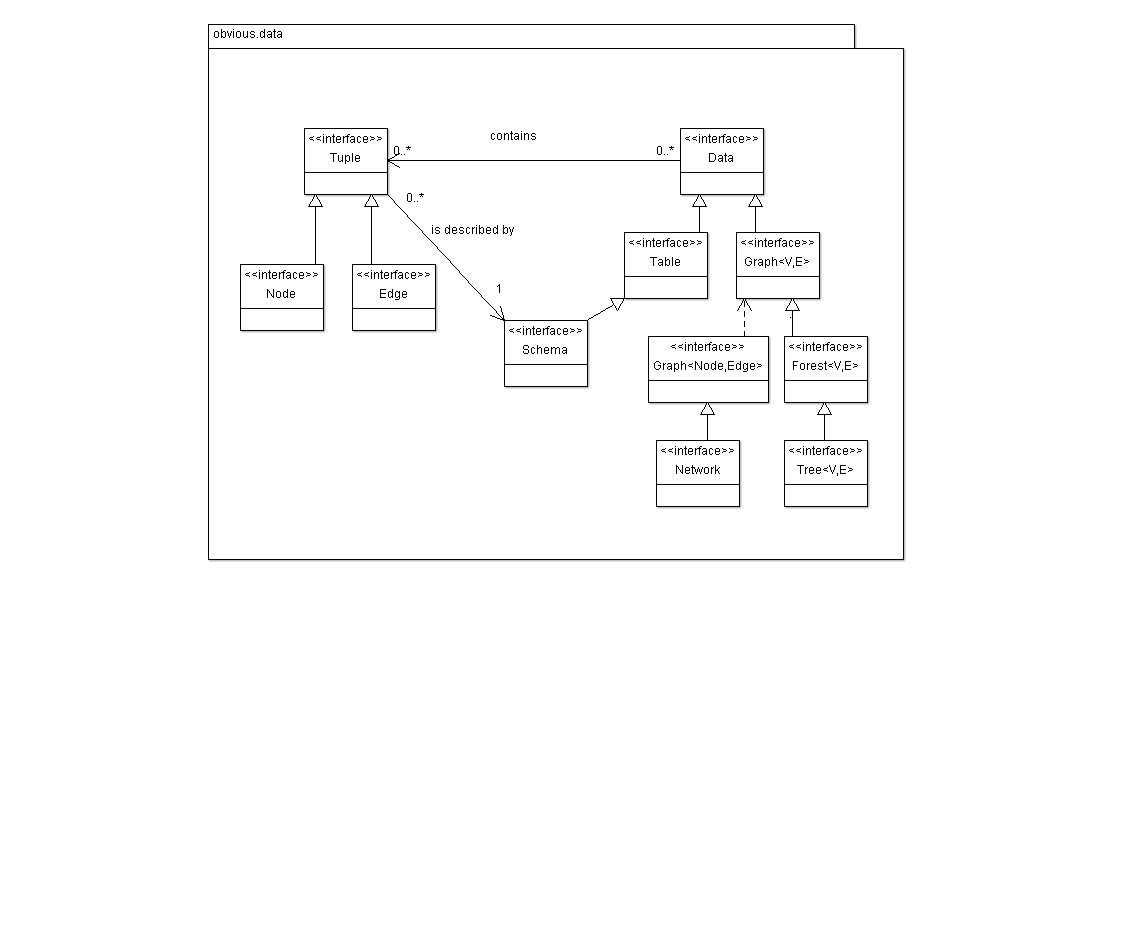
\includegraphics[width=\columnwidth]{figures/obviousdataclass}
\caption{Class diagram of the data model}
\label{fig:datamodel}
\end{figure}

The Obvious data model is centered on the proxy tuple design pattern
exposed in \cite{DesignPatternsIV}. Obvious adopts this design pattern
to offer high extensibility and good usability.  Among all the patterns
introduced in \cite{DesignPatternsIV}, the proxy tuple pattern enables
both as it encompasses graphs in an object-oriented manner --- many
developers are used to manipulation of \emph{object oriented graphs}
---- and as it unifies the data model around the same standard
structure (tuples and tables). In our data model, tuples are standards
elements of all structures: tables are composed of tuples and
graphs/trees are implemented as networks i.e. graphs built around two
tables one for the nodes and the other for the edges.

This model is instantiated via factories that allow cross-toolkit
interoperable data structure instantiation. With those factories, it
is possible to instantiate tables and networks from a schema or from
an existing object from a targeted Obvious implementation (e.g. a
Prefuse table or a JUNG graph). This also provides the possibility
to use parameters to provide more arguments used in targeted
toolkits. For example, in the Prefuse implementation of Obvious,
parameters are used to specify the source and target node columns for
a graph in an edge table.

In addition to data access, our data model allows providing 3
optional, interoperable, features: \emph{introspection}, \emph{batch
  editing} and \emph{notification}. Those features are not found in
all target toolkit implementations and thus sometimes had to be
emulated.
 
\subsubsection{Introspection}

Introspection means the capability of a program to inspect its own
content. In the context of the data model it means mostly that objects
expose their own schema explicitly and allow manipulating it as a
full-fledged object.  As an improvement over \cite{DesignPatternsIV},
our data model uses a meta-circular schema design (the schema is
itself a table) instead of a column object, that does not exist in
Obvious.  Schemas have been introduced because they are an efficient
an elegant mean to gather all \emph{meta-data} for the columns of a
table in one unique structure, allowing easy table and network
instantiations with a factory.  The main use of introspection in a
toolkit, though, is to enable generic implementation of a variety of
side services as varied as generic persistence, undo/redo, and
universal object editors.

\subsubsection{Batch Editing}

Batch editing means that one or many cells in a data model may be
edited at the same time.  This happens when the toolkit manages
analytical columns (e.g. computing the centrality of each vertex in a
network), with selection and dynamic queries if their effect is
reported to a data column or simply if a user wants to change values
interactively, either in the data table or through a visualization by
direct manipulation~\cite{Discovery3}.

\subsubsection{Notification}

All the popular infovis toolkits
(e.g. \cite{Prefuse, InfoVis, jung2003, Discovery1}) implement
notification using the ``Observer'' pattern from~\cite{DesignPatterns}
to propagate information about changes affecting the data model.  This
pattern specifies two roles: Observable and Observer; in our case,
data models are Observables meaning that the allow Observers to
register and be notified when they are changed.  During the design of
Obvious, we realized there were some variants in the way toolkits
implemented this pattern.  This is why the notification system
introduced in Obvious is designed to support a wide variety of
notification models, even those not currently implemented in current
toolkits but that will be required to scale.  The notification system
in Obvious is also based on the Observer design pattern with
extensions to supports transaction and batch techniques usually found
in database system.

%\subsubsection{Combining Notification and batch editing}
\label{sub:combiningnotif}

Combining Notification and batch editing raises a challenge: since one
operation can affect a large amount of data, a flow of notifications
concerning the same action will be generated.  If each change is
managed in isolation, the application can spend a large amount of time
updating visual structures, e.g. recomputing a layout for each
modified item.  This typically leads to the application being
unresponsive for a long time.

\begin{figure}[!ht]
  \centering
  
\includegraphics[width=.5\columnwidth]{figures/notification}

  \caption{Sequence diagram for the notification system}
  \label{fig:notification}
\end{figure}

Thus, Obvious introduces a method to control the management of batch
notifications: the \emph{beginEdit/endEdit} mechanism.
Figure~\ref{fig:notification} shows the sequence diagrams of the
notification manager.  Each time a data table is changed, the change
is transmitted to the Observer with a call to the \emph{tableChanged}
method.  This method takes several arguments describing the current
event (affected Table, rows, columns and operation type): this is the
typical Observer pattern.

When the \emph{beginEdit} method is called on an Obvious data table,
the Observer's \emph{beginEdit} method is called to start a batch
editing transaction.  Different strategies can be applied by the
observer.  A \emph{mode} parameter allows the observer to select a
specific strategy depending on the type of transaction (atomic or
batched).  Note that the observer will still receive a tableChanged
call for each tuple modified.  The observer is in charge of
implementing a strategy to optimize atomic/batch edition.  If it does
not, the standard behavior will happen and batch editing will flood
the observer --- which is acceptable in some cases.  The following
strategies have already been developed in one or more Obvious
implementations:

\begin{description}
\item[Lazy strategy] after a beginEdit, the observer ignores all the
  tableChanged calls until the endEdit method is called; then, the
  observer's actions are performed e.g. a layout is recomputed.

\item[Batch strategy] after beginEdit, the observer buffers the
  information sent by tableChanged.  When endEdit is called, the
  actions are performed on each of the buffered items.  Note that 
  buffering can be complicated when items are created, deleted or
  changed many times.  The burden is left to the observer since this
  management can be heavily optimized depending on the action to
  perform.

\item[Transaction strategy] after beginEdit, the observer buffers the
  information sent by tableChanged.  When endEdit is called, it first
  checks structural invariants (for example, no null value for a
  specific field) before performing its actions on the modified items.
\end{description}

The \emph{beginEdit/endEdit} mechanism has been added to support batch
editing and also database transactions.  When the data model
implementation relies on a transactional database, atomic and batch
transactions will occur and notifications (e.g. implemented as
database triggers) will arrive in batches.  The semantic of Obvious
notification handles this case correctly but the observer should be
aware that the tableChanged method can be called much later than when
the table is actually changed.  This is the case for database atomic
transactions: the actual notification is propagated after the end of
the transaction when the database engine has done all the integrity
checks.

In practice, the three strategies we have described have been
sufficient so far to handle all the cases required inside toolkits.
The impact on performance can be substantial, in particular to manage
dynamic data, a very standard situation in VA
applications that has not been well addressed in infovis so far.


\subsubsection{Other services}

To leverage our core implementation and offer some immediately useful
services to Obvious users, we have defined a utility package
``obviousx'', named in the same way as the Java extension package
``javax''.  This package provides different kinds of utility classes
for the Obvious data model.  First, we have defined reader and writer
interfaces allowing the creation of gateways between the Obvious data
model and common data formats such as CSV and GraphML.  It provides
software developers a standard way to import and export data in
Obvious whatever the underlying implementation of the data model
is.  In addition, for data providers, it simplifies their work because
they only have to develop one reader and one writer to be compatible
with a large number of toolkits.

With the same logic, obviousx provides compatibility classes to use
with standard Java components such as a Java Table Model that allows
the creation of a JTable from an Obvious table.  Finally, obviousx
also provides wrappers to \emph{map} obvious data structures into
common existing data structures (e.g. for Prefuse, IVTK, and Jung) to share data structures when using more than one
data model.

